\documentclass[UTF8]{ctexart}
\usepackage{geometry}
\geometry{margin=1.5cm, vmargin={0pt,1cm}}
\setlength{\topmargin}{-1cm}
\setlength{\paperheight}{29.7cm}
\setlength{\textheight}{25.3cm}

% useful packages.
\usepackage{amsfonts}
\usepackage{amsmath}
\usepackage{amssymb}
\usepackage{amsthm}
\usepackage{enumerate}
\usepackage{graphicx}
\usepackage{multicol}
\usepackage{fancyhdr}
\usepackage{layout}
\usepackage{float, caption}
\usepackage{xcolor}
\usepackage{listings}
\usepackage{tikz}

% 自定义配色方案,尽量模仿 VS Code 的高亮效果
\definecolor{codegreen}{rgb}{0,0.6,0}
\definecolor{codeblue}{rgb}{0,0,0.9}
\definecolor{codepurple}{rgb}{0.58,0,0.82}
\definecolor{codered}{rgb}{0.8,0,0}
\definecolor{backcolor}{rgb}{0.95,0.95,0.95}

% lstlisting 的风格设置
\lstdefinestyle{vscode}{
	backgroundcolor=\color{backcolor},   % 背景颜色
	commentstyle=\color{codegreen},     % 注释颜色
	keywordstyle=\color{codeblue}\bfseries, % 关键字颜色
	numberstyle=\tiny\color{gray},      % 行号颜色
	stringstyle=\color{codered},        % 字符串颜色
	basicstyle=\ttfamily\footnotesize,  % 基本字体
	breakatwhitespace=false,            % 仅在空格处断行
	breaklines=true,                    % 自动换行
	captionpos=b,                       % 标题位置(bottom)
	keepspaces=true,                    % 保持空格
	numbers=left,                       % 显示行号
	numbersep=5pt,                      % 行号与代码间的间隔
	rulecolor=\color{black},            % 框线颜色
	showspaces=false,                   % 不显示空格符号
	showstringspaces=false,             % 不显示字符串中的空格
	showtabs=false,                     % 不显示制表符
	frame=single,                       % 外框
	tabsize=4,                          % 制表符宽度
	escapeinside={(*@}{@*)},            % 特殊字符转义
	morekeywords={*,...}                % 添加更多自定义关键字
}
\lstset{style=vscode}

% some common command
\newcommand{\dif}{\mathrm{d}}
\newcommand{\avg}[1]{\left\langle #1 \right\rangle}
\newcommand{\difFrac}[2]{\frac{\dif #1}{\dif #2}}
\newcommand{\pdfFrac}[2]{\frac{\partial #1}{\partial #2}}
\newcommand{\OFL}{\mathrm{OFL}}
\newcommand{\UFL}{\mathrm{UFL}}
\newcommand{\fl}{\mathrm{fl}}
\newcommand{\op}{\odot}
\newcommand{\Eabs}{E_{\mathrm{abs}}}
\newcommand{\Erel}{E_{\mathrm{rel}}}

\begin{document}
	
	\pagestyle{fancy}
	\fancyhead{}
	\lhead{高凌溪, 3210105373}
	\chead{2024DS编程作业报告}
	\rhead{\today}
	\begin{abstract}
		本次编程作业主要利用\texttt{expression\_evaluator}类定义了一个简单运算的计算器,实现了加减乘除、负数、科学计数法和幂运算和对浮点数的中缀表达式求值。
	\end{abstract}
	\section{设计思路及实现原理}
	\begin{enumerate}
		\item 准备工作。根据用户的输入习惯,如果表达式中有空格,会先删除空格。其次用户输入负数的时候,必须以括号的形式输入,比如$(-1)+2$,而不是$-1+2$,这样一旦检测到表达式中有$(-$就会在负号之前插入$0$,比如$(-1)+2=(0-1)+2$。这一部分通过\texttt{modify()}函数实现。
		\item 定义运算符和优先级。以及各种运算符背后的具体运算,其中$\^$代表指数运算,比如$2\^3=2^3=8$;$e$代表科学计数法,比如$1.2e1=1.2\times10^1=12$。具体的成员函数如下:
		\begin{lstlisting}[language=C++, caption={运算符实现}, label={lst:operators}]
			bool isoperator(const char &c);
				if(c=='+' || c=='-' || c=='*' || c=='/' || c=='e' || c=='^'){
					return true;
				}
			int prior(const char &c);
			double calculate(const double &x, const double &y, const char &c) {
				if (c == 'e') {
					return x * pow(10, y);
				} else if (c == '^') {
					return pow(x, y);
				}
			}
		\end{lstlisting}
		\item 检查表达式是否合法。在运算之前先检查括号是否匹配和表达式是否合法,其中用栈来检测括号是否匹配,遇到左括号入栈,遇到右括号左括号出栈,最后检查栈是否为空。定义了以下两个公有成员函数
		\begin{lstlisting}[language=C++, caption={运算符实现}, label={lst:operators}]
		    bool isLegal(){
			int l=expressions.size();
			for(int i=0; i<l-1; ++i){
				bool a=!isdigit(expressions[i]) && expressions[i]!='(' && expressions[i]!=')';
				bool b=!isdigit(expressions[i+1])&& expressions[i+1]!='(' && expressions[i+1]!=')';
				bool c= expressions[i]=='.';
				bool d=expressions[i+1]=='.';
				if((i==0 && a ) || (i==l-2 && b ) ||
				(a && b) || (a&& expressions[i+1]==')')||(expressions[i]=='('&&expressions[i+1]==')')||
				(expressions[i]=='('&& b) ||(c && expressions[i+1]==')') ||(c && expressions[i+1]=='(') ||
				(expressions[i]=='(' && d) ||(expressions[i]==')' && d)||
				(expressions[i]=='(' && expressions[i+1]==')')){
					return false;
				}
			}
		\end{lstlisting}
		这会将括号不匹配、两个运算符直接相连(比如$2+-1$)、运算符出现在开头结尾(比如$-2+3$, $2*5/ \quad$,$3+(+1)\quad$,$2-(2*)$ )、小数点和运算符或者括号直接相连(比如$2.(3*4)\quad$,$3.+2\quad$,$(2+3).5$ )以及两个小数点(比如$1..2+1 \quad$,$1.2.1+2$ )、左右括号直接相连都看作不合法的表达式。但是$0021$这种以$0$开头的数字,是合法的,会舍弃掉多余的0.
		\item 计算。这会通过公有成员函数\texttt{evaluate()}实现,如果表达式不合法,会输出\texttt{brackets are matched or illegal expression}或者\texttt{invalid expression}来提示一个数字出现了多个小数点。一边生成后缀表达式一边计算。具体的,解析连续的数字或小数点,转换为双精度数压入数字栈;根据优先级规则处理操作符,必要时计算栈顶操作符的结果;通过括号分隔优先级不同的子表达式,计算并丢弃括号;遍历。
	\end{enumerate}
	\section{测试函数}
	\begin{enumerate}
		\item 设计了如下几个函数分别测试所有公有成员函数,包括表达式是否合法、括号匹配、处理浮点数、处理指数和科学计数法、处理负数和比较复杂的表达式计算。
		\begin{lstlisting}
			testModify();
			testIsLegal();
			testIsMatch();
			testEvaluate();
			testExponentiation();
			testNegativeNumbers();
			testFloatingPoint(); 
			testComprehensive(); 
			testDivideByZero();  
			testEmptyExpression();
		\end{lstlisting}
	\end{enumerate}
	\section{结果分析}
	最终测试的结果如下:
	\begin{lstlisting}
		g++ -o main main.cpp
		Running main:
		./main
		Test modify : ((-3)+4)*5 5
		----------------------------------------
		Test isLegal for valid expression 3 + 4 Pass
		Test isLegal for invalid expression +3 + 4 Fail
		Test isLegal for invalid expression 3 + + 4 Fail
		Test isLegal for invalid expression 3 + (4 * 2 Pass
		Test isLegal for invalid expression 3 + 4) * 2 Pass
		Test isLegal for invalid expression 3 + 4 * 2 +: Fail
		Test isLegal for invalid expression /3 + 4 * 2 + Fail
		Test isLegal for invalid expression 1..2+2 Fail
		Test isLegal for invalid expression (2+3).5 Fail
		Test isLegal for invalid expression 1.(2-1) Fail
		Test isLegal for invalid expression 3+()+2 Fail
		----------------------------------------
		Test isMatch for matching parentheses 3 + (4 * 2): Pass
		Test isMatch for unbalanced parentheses 3 + (4 * 2: Fail
		Test isMatch for matching parentheses 3 + 4 * (2 + 5): Pass
		Test isMatch for unbalanced parentheses 3 + 4 * 2): Fail
		----------------------------------------
		Test evaluate (3 + 4) = 7
		Test evaluate (5 * 6) = 30
		Test evaluate (10 / 2) = 5
		Test evaluate (2 * (3 + 4)) = 14
		Test evaluate (2 + 3 * 5) = 17
		Test evaluate (3 + 4) * 5 = 35
		Test evaluate invalid expression 10 ^ 3 = 1000
		Test evaluate 3 + (4 * 2) = 11
		Test evaluate 2.1e1+3^2-(-2)*3 = 36
		----------------------------------------
		Test exponentiation 2 e 3 = 2000
		Test exponentiation 5 e 2 = 500
		Test exponentiation 1 e 4 = 10000
		Test exponentiation 3 e 0 = 3
		----------------------------------------
		Test negative numbers ((-3) + 4) * 5 =5
		Test negative numbers (-3) + 4=1
		Test negative numbers 3 + (-4) =: -1
		----------------------------------------
		Test floating point numbers 3.5 + 4.2 =7.7
		Test floating point numbers 5.5 * 2 = 11
		Test floating point numbers 10.4 / 2 = 5.2
		----------------------------------------
		Test Comprehensive expression: 3 + 5 * 2 - 1= 12
		Test Comprehensive expression: (3+5)*(2-1)= 8
		Test Comprehensive expression: 2+3*(6/3)e1= 62
		Test Comprehensive expression: 4e2^0.5= 20
		Test Comprehensive expression: 0.08e(-1 )^(1/3) = 0.2
		Test Comprehensive expression: 0.21.1+2 = invalid expression
		-1
		Test Comprehensive expression: 0022+0.11e2-(-3)^2 = 24
		----------------------------------------
		Test divide by zero 10 / 0: can not be devided by zero
		-1
		----------------------------------------
		Test empty expression: no expression!
		-1
		
	\end{lstlisting}
	\section{设计的不足以及可能的改进方案}
	\begin{enumerate}
		\item 在我的设计中$-1+2$的这种情况将被判断为不合法的输入,如果要进行负数运算,必须要输入$(-1)+2$,然而在实际中第一种形式的表达式也往往不会引起误解并且被广泛应用。
		\item 在我的设计中,尽管实现了对科学计数法的运算,但本质上是将$e$看作了一种特殊的运算符,比如$2e3=2\times 10^3=2000$。但是在实际应用中,科学计数法往往要求形如$a \time 10^b$ 的形式,这里要求$1 \le a <2,\ b\in \mathbb{N}$,但是在我写的运算器中,形如$0.3e2.5$这样的运算也不会报错,这与实际的使用习惯不符。
		\item 最后是算法的效率问题。如果一个表达式是$(1+2)*(1+2)+(1+2)$,这将计算三次$1+2$,如果表达式非常长,这种重复计算相同的表达式显然是低效率的,为此一个可能的我认为的改进思路是使用有向图。下面举例说明:比如要计算$(a+b)-(a+b)/(c*(a+b))$,可以建立如下的有向图\\
		\begin{tikzpicture}[every node/.style={circle, draw, minimum size=1cm}, every path/.style={->, thick}]
			% Nodes
			\node (n1) at (0, 2) {$/$};
			\node (n2) at (-2, 1) {$+$};
			\node (n3) at (2, 1) {$*$};
			\node (n4) at (-3, 0) {$a$};
			\node (n5) at (-1,0) {$b$};
			\node (n6) at (3,0) {$c$};		
			\node (n7) at (-1,3) {$-$};
			% Edges
			\draw (n1) -- (n2);
			\draw (n1) -- (n3);
			\draw (n2) -- (n4);
			\draw (n2) -- (n5);
			\draw (n3) -- (n6);
			\draw (n3) -- (n2);
			\draw (n7) -- (n1);
			\draw (n7) -- (n2);
		\end{tikzpicture}
		\\
		然后利用逆拓扑排序,依次运算,但是这种方式可能存在的问题是$/\quad -$运算都是有左右之分的,但是有向无权图的节点连接的其他节点地位是相等的,因此这种方式更适合运算只有$+\quad *$的情况。
		
	\end{enumerate}
\end{document}
